% NLP Project 2: scientific extended abstract.
% CCN supplied 10pt, letter, two-column style. Two-page research body.
% AUTHOR ORDER AND STUDENT NUMBERS supplied by group on 26 October 2026.
% Ethics answers/contributions remain the named authors' responsibility.
\documentclass[10pt,letterpaper]{article}
\usepackage{ccn}
\usepackage{pslatex}
\usepackage[natbibapa]{apacite}
\usepackage{graphicx,booktabs,amsmath,microtype,xcolor,hyperref}
\hypersetup{hidelinks,pdftitle={When Sampling Shapes the Story: An Audit of Historical isiXhosa NLP},pdfauthor={Arno Strauss; Priyanka Gohil; Mohammed Bangie}}
\usepackage[labelfont=bf,font=sf,skip=2pt]{caption}
\setlength{\belowcaptionskip}{0pt}
\setlength{\abovecaptionskip}{1pt}
\newcommand{\answerYes}[1][]{\textbf{[Yes]} #1}
\newcommand{\answerNo}[1][]{\textbf{[No]} #1}
\newcommand{\answerNA}[1][]{\textbf{[N/A]} #1}
\newcommand{\answerTODO}[1][]{\textcolor{red}{\textbf{[REVIEW]}}}
\newcommand{\justificationTODO}[1][]{\textcolor{red}{\textbf{[AUTHOR REVIEW REQUIRED]}}}
\title{When Sampling Shapes the Story: Representation and Claim Reliability in Historical isiXhosa NLP}
\author{{\normalsize \bf Arno Strauss (2613224) \quad Priyanka Gohil (2586288) \quad Mohammed Bangie (2610990)}\\University of the Witwatersrand, Johannesburg, South Africa}
\date{}
\begin{document}
\maketitle
\vspace{-10pt}
\section{Abstract}
\noindent
Sampling is often treated as a neutral preprocessing step in historical-language NLP. We test whether it instead changes both \emph{model outcomes} and \emph{the conclusions researchers draw from texts}. In a controlled isiXhosa-newspaper study, fixed-budget BPE and Unigram tokenisers show improved English-view segmentation but less compact isiXhosa-view segmentation. We then introduce \emph{ArchiveLens}, an auditable workflow that tests historical surface-pattern trends under alternative sampling units, permutation calibration and repeated-text diagnostics. Although 23/120 Imvo patterns reverse estimated direction, the count is not unusual under permutation; 29 exhibit Holm-adjusted estimator-gap magnitude sensitivity. We argue that responsible historical NLP requires \emph{exposure-aware evaluation and calibrated claim warnings}, not assertions of cultural change from surface patterns.\\[-1pt]
\noindent\textbf{Keywords:} Responsible NLP; historical isiXhosa; sampling sensitivity; measurement validity.
\vspace{-4pt}
\section{Introduction and Related Work}
The \emph{same} historical newspaper text can yield different numerical descriptions depending on whether researchers count pages or words: in matched \emph{Imvo Zabantsundu} years, the archive's English-view share is \emph{22.64\% by equal page} versus \emph{29.47\% by word mass}. Neither is necessarily incorrect; each answers a different exposure question. Such choices matter especially when working with the isiXhosa Intellectual Traditions archive, whose digitised newspapers preserve historically important African writing without constituting a representative sample of speakers or beliefs \citep{schoots2023archive}.

Multilingual tokenisation can impose unequal computational costs \citep{petrov2023}, and its intrinsic efficiency need not predict downstream performance \citep{ali2024}. Historical collection audits highlight the influence of source composition \citep{beelen2025}, while data statements demand explicit populations and limitations \citep{bender2018}. Building on behavioural stress testing \citep{ribeiro2020}, we ask two connected but \emph{distinct} questions: \textbf{(Q1)} Can controlled sampling shift computational representation across archive views? \textbf{(Q2)} Can sampling choices also change the apparent \emph{descriptive trends} measured in historical text? We test Q1 with a factorial intervention and Q2 with our \emph{ArchiveLens} auditing instrument; we do not infer that tokenisers caused historical trends.

\section{Methods}
\textbf{Q1---intervene on model exposure.} In \emph{Imvo}, a $2\!\times\!2$ design varies (A) page- versus word-weighted allocation between English and isiXhosa archive views, and (B) page- versus word-weighted choice \emph{within} views (PP, PW, WP, WW). Across BPE and Unigram, four arms and five seeds, we fit 40 principal tokenisers (2,000-piece vocabulary), each on $\sim$500,000 alphabetic characters. Training uses 1885 and Jan--Sep 1887, validation Oct--Dec 1887 and evaluation 1888; 1889--94 is a diagnostic. We assess pieces per 100 alphabetic characters and smoothed count-bigram bits per character (BPC). Factorial contrasts are paired and average over the other factor; uncertainty resamples publication issues.

\textbf{Q2---audit claims about the archive.} ArchiveLens uses \emph{Imvo} and \emph{Isigidimi samaXosa}, selecting 120 common within-word character four-grams by frequency in \emph{1887 only}. For 1888 minus 1885, it contrasts character-position mass, equal-page, equal-issue and equal-month rates (per 10,000 eligible four-gram positions). A 3,000-draw month/issue bootstrap describes uncertainty. We then calibrate direction-reversal counts and estimator-gap magnitudes using 4,999 within-month, whole-issue year-label permutations; Holm adjustment tests 120 patterns per source and statistic family. Leave-one-issue-out influence and exact cross-issue 13-word repetition masking probe sensitivity. These \emph{post-hoc conditional} analyses use previously inspected years, not independent external confirmation.

\begin{figure*}[t]
\centering
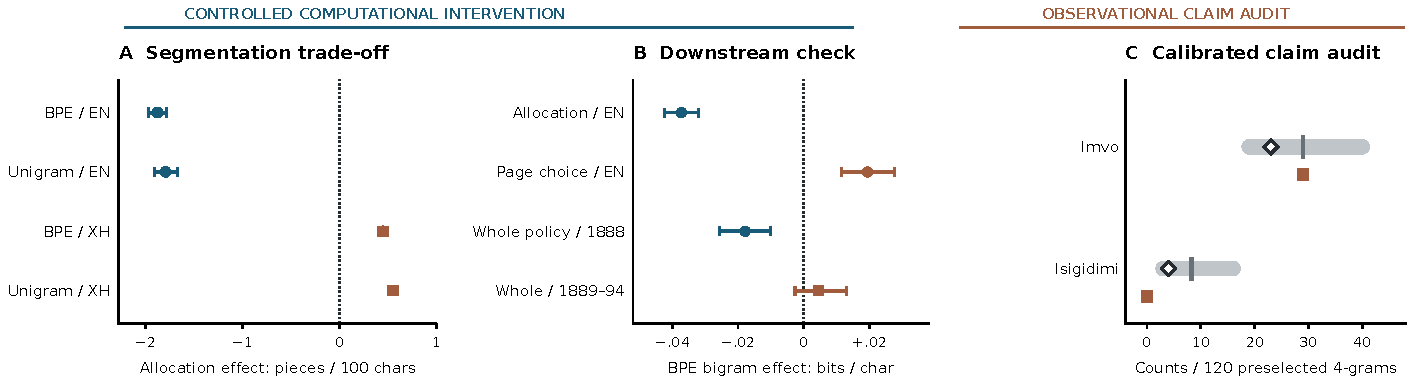
\includegraphics[width=.995\textwidth]{figures/integrated_evidence.pdf}
\vspace{-2pt}
\caption{\textbf{Two linked Responsible NLP failure modes.} \textbf{A:} 1888 allocation effects on segmentation for archive English (EN) and isiXhosa (XH) views; points and lines show 95\% issue-bootstrap intervals (negative = more compact). \textbf{B:} BPE English-view count-bigram effects for allocation, within-view page choice and combined policy (1888 issue intervals; 1889--94 whole-policy effect has a six-year interval). \textbf{C:} ArchiveLens's observed sign-reversal counts (hollow diamonds) versus whole-issue permutation means (grey ticks) and 95\% reference ranges (grey lines); coloured squares show \emph{different} Holm-adjusted tests of estimator-gap \emph{magnitude}. A sign reversal alone is not evidence of a historical semantic change.}
\label{fig:integrated}
\end{figure*}

\section{Results}
\textbf{Sampling changes what the model learns (Fig.~\ref{fig:integrated}A).} Changing allocation lowers English-view BPE segmentation cost by $1.878$ pieces/100 characters (signed $\Delta=-1.878$, 95\% issue CI $[-1.972,-1.782]$), but raises isiXhosa-view cost by $0.453$ (CI $[0.407,0.497]$). Unigram shows the same directional trade-off ($-1.795$ EN; $+0.555$ XH). \emph{The gain is not language-view-neutral.}

\textbf{Model utility is a second decision (Fig.~\ref{fig:integrated}B).} For English-view BPE, allocation improves bigram loss by $-0.0372$ BPC (95\% issue CI $[-0.0424,-0.0321]$), while within-view page choice worsens it by $+0.0194$ BPC (CI $[0.0115,0.0277]$). The combined policy improves 1888 BPC ($-0.0178$) but is \emph{inconclusive} in 1889--94 ($+0.0045$, six-year CI $[-0.0027,0.0131]$). Notably, isiXhosa-view BPE segmentation gets less compact while its average BPC improves slightly ($-0.00275$): intrinsic compactness is not a sufficient downstream proxy.

\textbf{Audit the warning itself (Fig.~\ref{fig:integrated}C).} Under alternative estimands, 23/120 \emph{Imvo} and 4/120 \emph{Isigidimi} four-gram trends reverse point-estimate sign, but none shows supported opposite directions under both estimands. Imvo's reversal \emph{count} is not unusual under 4,999 permutations (23 observed; null mean 29.0; upper-tail $p=.888$). In contrast, \emph{estimator-gap magnitude} survives Holm correction for 29/120 Imvo patterns (0/120 Isigidimi). Removing one issue reverses the mass-weighted sign in 7/32 flagged Imvo patterns; masking exact repeated passages eliminates 10 of Imvo's original 23 reversal warnings, while changing sample eligibility.

\section{Discussion: Responsible NLP}
\textbf{An algorithm can optimise the wrong denominator.} A language-averaged segmentation score hides the empirically opposed view-specific effects. Even a per-view segmentation gain cannot replace task-level measurement: allocation and page-choice effects oppose one another for English bigram loss, and isiXhosa BPC can move differently from compactness. Responsible evaluation must state the target exposure distribution \emph{before} declaring one policy better.

\textbf{A warning is not a discovery.} ArchiveLens makes the analysis denominator visible and tests the reliability of its own alerts. The negative result---no excess of raw reversal counts under the permutation reference---guards against exaggeration. Corrected estimator-gap tests nevertheless find measurable sensitivity in Imvo, while issue influence and repeated text explain why additional checks are needed. They do not identify historical causes; removing duplicated material alters the evaluated population. Isigidimi contains fewer issues (12 in 1888 versus Imvo's 52), so zero Holm-positive gaps must not be construed as a more reliable or fairer archive.

\textbf{From warning to accountable practice.} Instead of assigning an unexplained ``fairness score'', ArchiveLens records each tested statement's source and dates, its denominator and alternative estimands, issue-based uncertainty, calibration reference, and influential or repeated text. A defensible reporting rule is to describe a result as \emph{stable under tested assumptions}, \emph{measurement-sensitive}, or \emph{unresolved}; none of these labels certifies cultural truth. This matters when an apparently precise estimate might later inform search, access to collections or interpretations of political writing.\par

\textbf{Costs of misinterpretation.} Treating a short character sequence as a historical concept, or an archive view as an individual's language, could misrepresent the people represented by the collection. Our audit can flag this technical risk but cannot resolve it. Further work needs language experts and archivists to validate meaningful word forms, editorial context and intended applications, alongside independent corpora and community-grounded assessment.\par

\textbf{Limits and responsible use.} \texttt{EnTxt}/\texttt{XhTxt} are archive views, not human-validated word-language identities. The files are corrected transcriptions, not raw-OCR confidence annotations; genre, editorial practice, preservation and earlier analyst exposure to test years remain confounders. Four-grams are surface strings, not morphemes or cultural ideas, and both newspapers share one source collection. We neither measure societal fairness harm nor establish historical semantic change. Human linguistic/archival review and genuinely external evaluation are needed before those claims.

\section{Conclusion}
\emph{Which texts are exposed, which outcome is optimised, and which claims survive counterfactual weighting} are inseparable parts of responsible historical NLP. Our controlled study and calibrated ArchiveLens workflow make these choices empirically visible and reproducible. Source, tests, frozen protocols and full evidence are in the \href{https://github.com/Stralb/isixhosa-archive-nlp/blob/main/reports/PAPER_TO_EVIDENCE_GUIDE.md}{open research repository}.

\clearpage
\bibliographystyle{apacite}
\bibliography{paper_references}
\clearpage
\section*{NeurIPS Paper Checklist}




\begin{enumerate}

\item {\bf Claims}
    \item[] Question: Do the main claims made in the abstract and introduction accurately reflect the paper's contributions and scope?
    \item[] Answer: \answerYes{}
    \item[] Justification: Sections 1--5 describe the two distinct analyses, effects and boundaries.
    \item[] Guidelines:
    \begin{itemize}
        \item The answer NA means that the abstract and introduction do not include the claims made in the paper.
        \item The abstract and/or introduction should clearly state the claims made, including the contributions made in the paper and important assumptions and limitations. A No or NA answer to this question will not be perceived well by the reviewers. 
        \item The claims made should match theoretical and experimental results, and reflect how much the results can be expected to generalize to other settings. 
        \item It is fine to include aspirational goals as motivation as long as it is clear that these goals are not attained by the paper. 
    \end{itemize}

\item {\bf Limitations}
    \item[] Question: Does the paper discuss the limitations of the work performed by the authors?
    \item[] Answer: \answerYes{}
    \item[] Justification: The paper names reused years, proxy view labels, source/genre confounding, repetition and cultural-interpretation limits.
    \item[] Guidelines:
    \begin{itemize}
        \item The answer NA means that the paper has no limitation while the answer No means that the paper has limitations, but those are not discussed in the paper. 
        \item The authors are encouraged to create a separate "Limitations" section in their paper.
        \item The paper should point out any strong assumptions and how robust the results are to violations of these assumptions (e.g., independence assumptions, noiseless settings, model well-specification, asymptotic approximations only holding locally). The authors should reflect on how these assumptions might be violated in practice and what the implications would be.
        \item The authors should reflect on the scope of the claims made, e.g., if the approach was only tested on a few datasets or with a few runs. In general, empirical results often depend on implicit assumptions, which should be articulated.
        \item The authors should reflect on the factors that influence the performance of the approach. For example, a facial recognition algorithm may perform poorly when image resolution is low or images are taken in low lighting. Or a speech-to-text system might not be used reliably to provide closed captions for online lectures because it fails to handle technical jargon.
        \item The authors should discuss the computational efficiency of the proposed algorithms and how they scale with dataset size.
        \item If applicable, the authors should discuss possible limitations of their approach to address problems of privacy and fairness.
        \item While the authors might fear that complete honesty about limitations might be used by reviewers as grounds for rejection, a worse outcome might be that reviewers discover limitations that aren't acknowledged in the paper. The authors should use their best judgment and recognize that individual actions in favor of transparency play an important role in developing norms that preserve the integrity of the community. Reviewers will be specifically instructed to not penalize honesty concerning limitations.
    \end{itemize}

\item {\bf Theory Assumptions and Proofs}
    \item[] Question: For each theoretical result, does the paper provide the full set of assumptions and a complete (and correct) proof?
    \item[] Answer: \answerNA{}
    \item[] Justification: The paper presents no theorem or formal proof; findings are empirical.
    \item[] Guidelines:
    \begin{itemize}
        \item The answer NA means that the paper does not include theoretical results. 
        \item All the theorems, formulas, and proofs in the paper should be numbered and cross-referenced.
        \item All assumptions should be clearly stated or referenced in the statement of any theorems.
        \item The proofs can either appear in the main paper or the supplemental material, but if they appear in the supplemental material, the authors are encouraged to provide a short proof sketch to provide intuition. 
        \item Inversely, any informal proof provided in the core of the paper should be complemented by formal proofs provided in appendix or supplemental material.
        \item Theorems and Lemmas that the proof relies upon should be properly referenced. 
    \end{itemize}

    \item {\bf Experimental Result Reproducibility}
    \item[] Question: Does the paper fully disclose all the information needed to reproduce the main experimental results of the paper to the extent that it affects the main claims and/or conclusions of the paper (regardless of whether the code and data are provided or not)?
    \item[] Answer: \answerYes{}
    \item[] Justification: The public repository contains scripts, source hashes, fixed seeds, resampling rules and independent verifiers.
    \item[] Guidelines:
    \begin{itemize}
        \item The answer NA means that the paper does not include experiments.
        \item If the paper includes experiments, a No answer to this question will not be perceived well by the reviewers: Making the paper reproducible is important, regardless of whether the code and data are provided or not.
        \item If the contribution is a dataset and/or model, the authors should describe the steps taken to make their results reproducible or verifiable. 
        \item Depending on the contribution, reproducibility can be accomplished in various ways. For example, if the contribution is a novel architecture, describing the architecture fully might suffice, or if the contribution is a specific model and empirical evaluation, it may be necessary to either make it possible for others to replicate the model with the same dataset, or provide access to the model. In general. releasing code and data is often one good way to accomplish this, but reproducibility can also be provided via detailed instructions for how to replicate the results, access to a hosted model (e.g., in the case of a large language model), releasing of a model checkpoint, or other means that are appropriate to the research performed.
        \item While NeurIPS does not require releasing code, the conference does require all submissions to provide some reasonable avenue for reproducibility, which may depend on the nature of the contribution. For example
        \begin{enumerate}
            \item If the contribution is primarily a new algorithm, the paper should make it clear how to reproduce that algorithm.
            \item If the contribution is primarily a new model architecture, the paper should describe the architecture clearly and fully.
            \item If the contribution is a new model (e.g., a large language model), then there should either be a way to access this model for reproducing the results or a way to reproduce the model (e.g., with an open-source dataset or instructions for how to construct the dataset).
            \item We recognize that reproducibility may be tricky in some cases, in which case authors are welcome to describe the particular way they provide for reproducibility. In the case of closed-source models, it may be that access to the model is limited in some way (e.g., to registered users), but it should be possible for other researchers to have some path to reproducing or verifying the results.
        \end{enumerate}
    \end{itemize}


\item {\bf Open access to data and code}
    \item[] Question: Does the paper provide open access to the data and code, with sufficient instructions to faithfully reproduce the main experimental results, as described in supplemental material?
    \item[] Answer: \answerYes{}
    \item[] Justification: Source and derived materials are publicly visible in the repository, subject to verification of original archive redistribution permission.
    \item[] Guidelines:
    \begin{itemize}
        \item The answer NA means that paper does not include experiments requiring code.
        \item Please see the NeurIPS code and data submission guidelines (\url{https://nips.cc/public/guides/CodeSubmissionPolicy}) for more details.
        \item While we encourage the release of code and data, we understand that this might not be possible, so “No” is an acceptable answer. Papers cannot be rejected simply for not including code, unless this is central to the contribution (e.g., for a new open-source benchmark).
        \item The instructions should contain the exact command and environment needed to run to reproduce the results. See the NeurIPS code and data submission guidelines (\url{https://nips.cc/public/guides/CodeSubmissionPolicy}) for more details.
        \item The authors should provide instructions on data access and preparation, including how to access the raw data, preprocessed data, intermediate data, and generated data, etc.
        \item The authors should provide scripts to reproduce all experimental results for the new proposed method and baselines. If only a subset of experiments are reproducible, they should state which ones are omitted from the script and why.
        \item At submission time, to preserve anonymity, the authors should release anonymized versions (if applicable).
        \item Providing as much information as possible in supplemental material (appended to the paper) is recommended, but including URLs to data and code is permitted.
    \end{itemize}


\item {\bf Experimental Setting/Details}
    \item[] Question: Does the paper specify all the training and test details (e.g., data splits, hyperparameters, how they were chosen, type of optimizer, etc.) necessary to understand the results?
    \item[] Answer: \answerYes{}
    \item[] Justification: The Methods section identifies sampling arms, tokenizer families, dates, seeds, budgets and outcomes.
    \item[] Guidelines:
    \begin{itemize}
        \item The answer NA means that the paper does not include experiments.
        \item The experimental setting should be presented in the core of the paper to a level of detail that is necessary to appreciate the results and make sense of them.
        \item The full details can be provided either with the code, in appendix, or as supplemental material.
    \end{itemize}

\item {\bf Experiment Statistical Significance}
    \item[] Question: Does the paper report error bars suitably and correctly defined or other appropriate information about the statistical significance of the experiments?
    \item[] Answer: \answerYes{}
    \item[] Justification: Issue-level bootstrap intervals and whole-issue, within-month permutation tests are reported with caveats.
    \item[] Guidelines:
    \begin{itemize}
        \item The answer NA means that the paper does not include experiments.
        \item The authors should answer "Yes" if the results are accompanied by error bars, confidence intervals, or statistical significance tests, at least for the experiments that support the main claims of the paper.
        \item The factors of variability that the error bars are capturing should be clearly stated (for example, train/test split, initialization, random drawing of some parameter, or overall run with given experimental conditions).
        \item The method for calculating the error bars should be explained (closed form formula, call to a library function, bootstrap, etc.)
        \item The assumptions made should be given (e.g., Normally distributed errors).
        \item It should be clear whether the error bar is the standard deviation or the standard error of the mean.
        \item It is OK to report 1-sigma error bars, but one should state it. The authors should preferably report a 2-sigma error bar than state that they have a 96\% CI, if the hypothesis of Normality of errors is not verified.
        \item For asymmetric distributions, the authors should be careful not to show in tables or figures symmetric error bars that would yield results that are out of range (e.g. negative error rates).
        \item If error bars are reported in tables or plots, The authors should explain in the text how they were calculated and reference the corresponding figures or tables in the text.
    \end{itemize}

\item {\bf Experiments Compute Resources}
    \item[] Question: For each experiment, does the paper provide sufficient information on the computer resources (type of compute workers, memory, time of execution) needed to reproduce the experiments?
    \item[] Answer: \answerNo{}
    \item[] Justification: Detailed hardware/runtime and total exploratory-compute accounting have not been independently reconstructed; repository job logs provide partial traceability.
    \item[] Guidelines:
    \begin{itemize}
        \item The answer NA means that the paper does not include experiments.
        \item The paper should indicate the type of compute workers CPU or GPU, internal cluster, or cloud provider, including relevant memory and storage.
        \item The paper should provide the amount of compute required for each of the individual experimental runs as well as estimate the total compute. 
        \item The paper should disclose whether the full research project required more compute than the experiments reported in the paper (e.g., preliminary or failed experiments that didn't make it into the paper). 
    \end{itemize}
    
\item {\bf Code Of Ethics}
    \item[] Question: Does the research conducted in the paper conform, in every respect, with the NeurIPS Code of Ethics \url{https://neurips.cc/public/EthicsGuidelines}?
    \item[] Answer: \answerTODO{}
    \item[] Justification: AUTHOR ACTION: Review the actual NeurIPS Code of Ethics and verify compliance, licensing, attribution and release responsibilities.
    \item[] Guidelines:
    \begin{itemize}
        \item The answer NA means that the authors have not reviewed the NeurIPS Code of Ethics.
        \item If the authors answer No, they should explain the special circumstances that require a deviation from the Code of Ethics.
        \item The authors should make sure to preserve anonymity (e.g., if there is a special consideration due to laws or regulations in their jurisdiction).
    \end{itemize}


\item {\bf Broader Impacts}
    \item[] Question: Does the paper discuss both potential positive societal impacts and negative societal impacts of the work performed?
    \item[] Answer: \answerYes{}
    \item[] Justification: The Discussion identifies potential benefits and risks of applying surface metrics to culturally important archives.
    \item[] Guidelines:
    \begin{itemize}
        \item The answer NA means that there is no societal impact of the work performed.
        \item If the authors answer NA or No, they should explain why their work has no societal impact or why the paper does not address societal impact.
        \item Examples of negative societal impacts include potential malicious or unintended uses (e.g., disinformation, generating fake profiles, surveillance), fairness considerations (e.g., deployment of technologies that could make decisions that unfairly impact specific groups), privacy considerations, and security considerations.
        \item The conference expects that many papers will be foundational research and not tied to particular applications, let alone deployments. However, if there is a direct path to any negative applications, the authors should point it out. For example, it is legitimate to point out that an improvement in the quality of generative models could be used to generate deepfakes for disinformation. On the other hand, it is not needed to point out that a generic algorithm for optimizing neural networks could enable people to train models that generate Deepfakes faster.
        \item The authors should consider possible harms that could arise when the technology is being used as intended and functioning correctly, harms that could arise when the technology is being used as intended but gives incorrect results, and harms following from (intentional or unintentional) misuse of the technology.
        \item If there are negative societal impacts, the authors could also discuss possible mitigation strategies (e.g., gated release of models, providing defenses in addition to attacks, mechanisms for monitoring misuse, mechanisms to monitor how a system learns from feedback over time, improving the efficiency and accessibility of ML).
    \end{itemize}
    
\item {\bf Safeguards}
    \item[] Question: Does the paper describe safeguards that have been put in place for responsible release of data or models that have a high risk for misuse (e.g., pretrained language models, image generators, or scraped datasets)?
    \item[] Answer: \answerNo{}
    \item[] Justification: Archival text is publicly redistributed in this repository; authoritative transcription redistribution rights must be confirmed by the authors.
    \item[] Guidelines:
    \begin{itemize}
        \item The answer NA means that the paper poses no such risks.
        \item Released models that have a high risk for misuse or dual-use should be released with necessary safeguards to allow for controlled use of the model, for example by requiring that users adhere to usage guidelines or restrictions to access the model or implementing safety filters. 
        \item Datasets that have been scraped from the Internet could pose safety risks. The authors should describe how they avoided releasing unsafe images.
        \item We recognize that providing effective safeguards is challenging, and many papers do not require this, but we encourage authors to take this into account and make a best faith effort.
    \end{itemize}

\item {\bf Licenses for existing assets}
    \item[] Question: Are the creators or original owners of assets (e.g., code, data, models), used in the paper, properly credited and are the license and terms of use explicitly mentioned and properly respected?
    \item[] Answer: \answerNo{}
    \item[] Justification: The archive and several software packages are credited, but the original archive redistribution permission still needs confirmation.
    \item[] Guidelines:
    \begin{itemize}
        \item The answer NA means that the paper does not use existing assets.
        \item The authors should cite the original paper that produced the code package or dataset.
        \item The authors should state which version of the asset is used and, if possible, include a URL.
        \item The name of the license (e.g., CC-BY 4.0) should be included for each asset.
        \item For scraped data from a particular source (e.g., website), the copyright and terms of service of that source should be provided.
        \item If assets are released, the license, copyright information, and terms of use in the package should be provided. For popular datasets, \url{paperswithcode.com/datasets} has curated licenses for some datasets. Their licensing guide can help determine the license of a dataset.
        \item For existing datasets that are re-packaged, both the original license and the license of the derived asset (if it has changed) should be provided.
        \item If this information is not available online, the authors are encouraged to reach out to the asset's creators.
    \end{itemize}

\item {\bf New Assets}
    \item[] Question: Are new assets introduced in the paper well documented and is the documentation provided alongside the assets?
    \item[] Answer: \answerYes{}
    \item[] Justification: The new ArchiveLens code, protocols, examples and limitations are described and independently tested in the repository.
    \item[] Guidelines:
    \begin{itemize}
        \item The answer NA means that the paper does not release new assets.
        \item Researchers should communicate the details of the dataset/code/model as part of their submissions via structured templates. This includes details about training, license, limitations, etc. 
        \item The paper should discuss whether and how consent was obtained from people whose asset is used.
        \item At submission time, remember to anonymize your assets (if applicable). You can either create an anonymized URL or include an anonymized zip file.
    \end{itemize}

\item {\bf Crowdsourcing and Research with Human Subjects}
    \item[] Question: For crowdsourcing experiments and research with human subjects, does the paper include the full text of instructions given to participants and screenshots, if applicable, as well as details about compensation (if any)? 
    \item[] Answer: \answerNA{}
    \item[] Justification: No new participants were recruited, surveyed, annotated or subjected to experiments.
    \item[] Guidelines:
    \begin{itemize}
        \item The answer NA means that the paper does not involve crowdsourcing nor research with human subjects.
        \item Including this information in the supplemental material is fine, but if the main contribution of the paper involves human subjects, then as much detail as possible should be included in the main paper. 
        \item According to the NeurIPS Code of Ethics, workers involved in data collection, curation, or other labor should be paid at least the minimum wage in the country of the data collector. 
    \end{itemize}

\item {\bf Institutional Review Board (IRB) Approvals or Equivalent for Research with Human Subjects}
    \item[] Question: Does the paper describe potential risks incurred by study participants, whether such risks were disclosed to the subjects, and whether Institutional Review Board (IRB) approvals (or an equivalent approval/review based on the requirements of your country or institution) were obtained?
    \item[] Answer: \answerNA{}
    \item[] Justification: No research involving recruited living human subjects was conducted; authors should verify the institution's position on archival data.
    \item[] Guidelines:
    \begin{itemize}
        \item The answer NA means that the paper does not involve crowdsourcing nor research with human subjects.
        \item Depending on the country in which research is conducted, IRB approval (or equivalent) may be required for any human subjects research. If you obtained IRB approval, you should clearly state this in the paper. 
        \item We recognize that the procedures for this may vary significantly between institutions and locations, and we expect authors to adhere to the NeurIPS Code of Ethics and the guidelines for their institution. 
        \item For initial submissions, do not include any information that would break anonymity (if applicable), such as the institution conducting the review.
    \end{itemize}

\end{enumerate}

\clearpage
\section*{Faculty of Science AI Ethics Statement---author approval required}
\noindent\textbf{Proposed factual disclosure for author review:} Generative AI assisted literature organisation, paper wording, source-code review and typesetting. Human authors must verify and take responsibility for every scientific claim, the research methodology, data-rights decisions and final submission. This note does not replace the official Faculty form or mandatory declaration.\\[5pt]
\noindent\textbf{AUTHORS:} Insert and complete the official University of the Witwatersrand Faculty of Science AI Ethics statement as required by the module. Verify the final wording, permissions, and signatures.

\section*{Contribution Statement---author approval required}
\noindent\textbf{Arno Strauss (2613224), Priyanka Gohil (2586288), Mohammed Bangie (2610990):} authors must record their truthful individual contributions and approve the final text. No responsibilities or contribution percentages are inferred from author ordering.
\end{document}
